%!TEX TS-program=pdflatex
%!TEX encoding=latin1
%%%%%%%%
% This introduction to LaTeX by Christian Mueller and Nicolas Zahn is licensed
% under the Creative Commons Attribution-ShareAlike 3.0 Unported License. To view
% a copy of this license, visit http://creativecommons.org/licenses/by-sa/3.0/
% or send a letter to Creative Commons, 444 Castro Street, Suite 900, Mountain
% View, California, 94041, USA.
%%%%%%%%
% title: Einfache Pr�sentation mit der "beamer"-Klasse
% author: Christian Mueller
% last changed: 2011-11-01
%%%%%%%%
\documentclass[12pt]{beamer}

%%% additional required packages %%%
\usepackage[latin1]{inputenc} % input scheme for windows
\usepackage[T1]{fontenc} % font encoding for windows
\usepackage{graphicx} % graphics support for LaTeX
\usepackage[UKenglish]{babel} % multilingual support for LaTeX


%%% some formatting stuff %%%
% set the overall look of the slides %
\setbeamertemplate{frametitle}[default][right]
\useinnertheme{default}
\setbeamercovered{transparent}
% additional customisation of the look of the slides %
\setbeamerfont{framesubtitle}{size=\large}

% the font to use %
\usepackage{lmodern}


%%% title information %%%
\title{Applied Statistics Using R}
% \subtitle{}
\author{Christian M�ller}
\date{April 1, 2010}
\institute{Seminar Presentations in English -- Arts and Social Sciences}


%%%%%%%%%%%%%%%%%%%%%%%%%%%%%%%
%% Hier beginnt das Dokument %%
%%%%%%%%%%%%%%%%%%%%%%%%%%%%%%%

\begin{document}

\begin{frame}
\titlepage
\end{frame}


\section*{Table of Contents}

\begin{frame}
\frametitle{Table of Contents}
\tableofcontents
\end{frame}


\section{Why using R?}

\begin{frame}
\frametitle{Why using R?}
\framesubtitle{Some Reasons}

\begin{itemize}[<+->]
    \item You want to use sophisticated quantitative methods
  \item You want to apply statistics in innovative ways
    \item You need a statistical package that can keep up with you
    \item R is your statistical package of choice
\end{itemize}

\end{frame}


\begin{frame}
\frametitle{Why using R?}
\framesubtitle{}

\begin{itemize}[<+->]
    \item R is maintained and constantly advanced by some of the most renowned statisticians worldwide
    \item Many additional packages and extension are available
    \item R is FREE! (GNU-GPL)
    \item R is a joint project of applied statisticians for applied statisticians
\end{itemize}

\end{frame}


\begin{frame}
\frametitle{Why using R?}
\framesubtitle{Advantages and Disadvantages}

\begin{columns}[t]
    \column{.5\textwidth}<1->
        \begin{block}{Advantages}
        \begin{itemize}
        \item extremely flexible
        \item highly programmable
        \item you can do much more than standard, pre-canned analysis
        \end{itemize}
    \end{block}
    
    \column{.5\textwidth}<2->
        \begin{block}{Disadvantages}
        \begin{itemize}
        \item harder to learn than other statistical packages
        \item scant documentation
        \item you should have some statistical background
        \end{itemize}
        \end{block}
\end{columns}

\end{frame}



\section{Applied Example}

\begin{frame}
\frametitle{Applied Example}
\framesubtitle{Solving a sudoku}

\centering
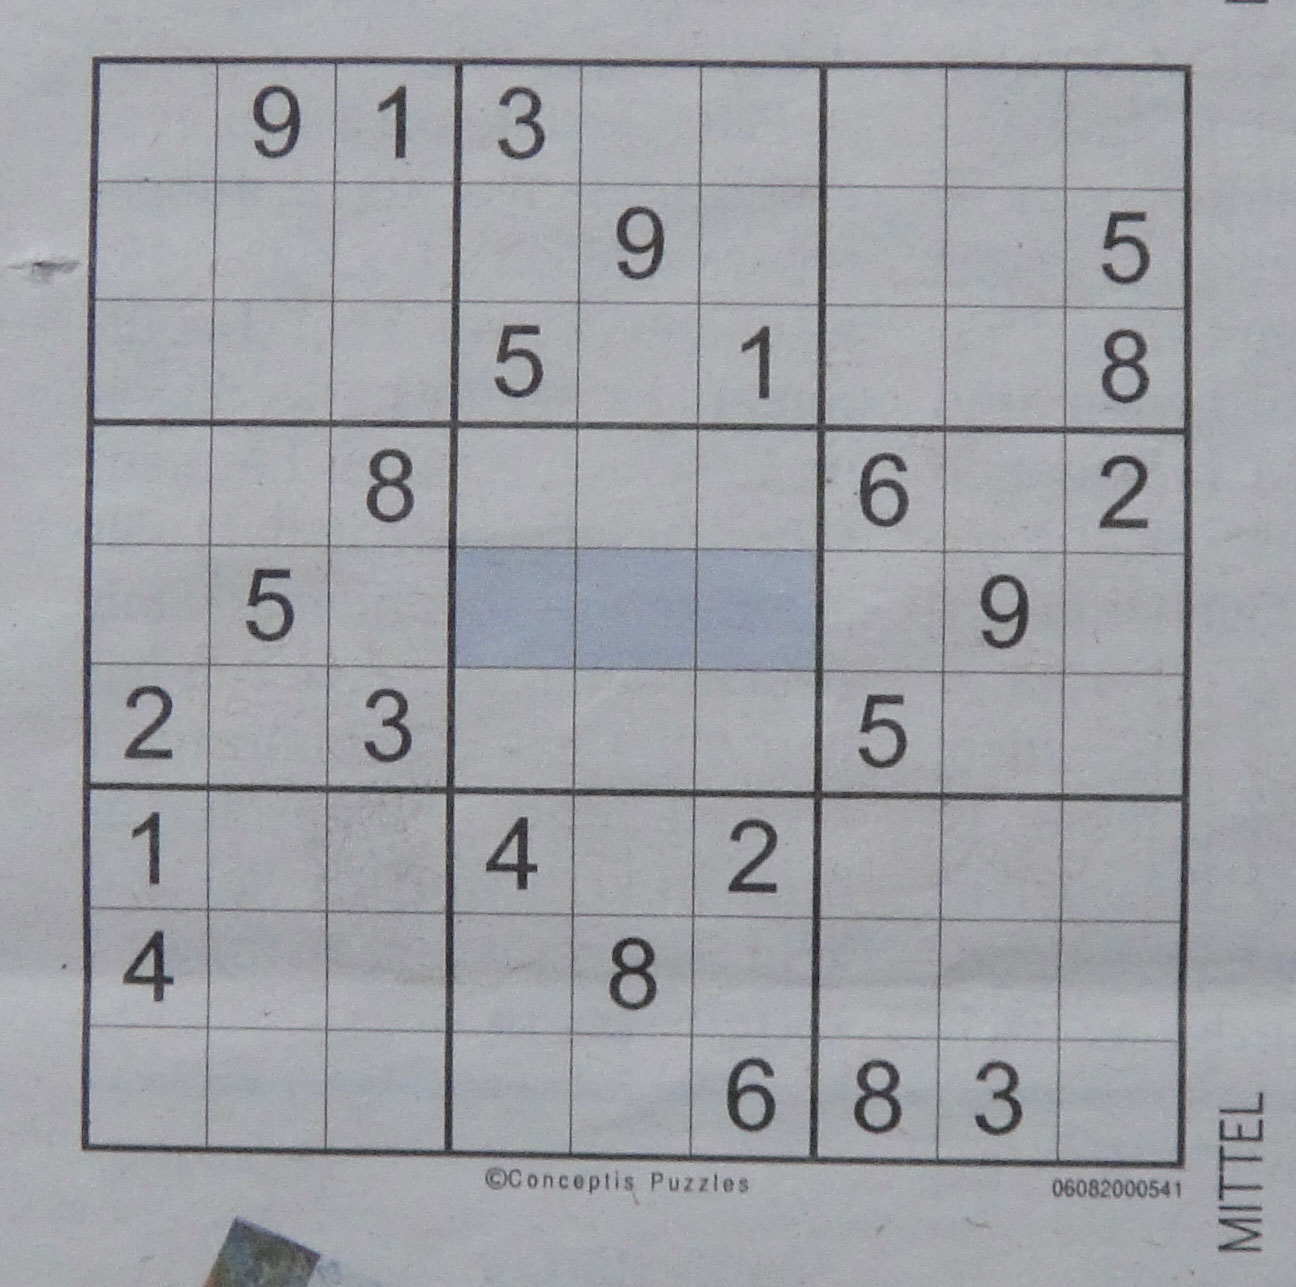
\includegraphics[width=0.5\textwidth]{sudoku_leer.jpg}

\vfill

\hfill \scriptsize{source: 20 Minuten, 30.3.2010.}

\end{frame}




\begin{frame}
\frametitle{Applied Example}
\framesubtitle{Solving a sudoku}

\begin{itemize}
    \item Mathematically there are a number of different methods:
    \begin{itemize}
        \item<2-> Cultural Genetic Algorithm (CGA)
        \item<2-> \textbf<3->{\structure<3->{Simulated Annealing (SA)}}
        \item<2-> Quantum Simulated Annealing (QSA)
        \item<2-> Hybrid method combining Genetic Algorithm with Simulated Annealing (HGASA)
    \end{itemize}
    
\end{itemize}

\end{frame}


\begin{frame}[fragile]
\frametitle{Applied Example}
\framesubtitle{Solving a sudoku}

\footnotesize
\begin{verbatim}
    # target function to minimise
    # that counts lines+rows+blocks
    # missing the no duplicate constraint
    target=function(s){
      tar=sum(apply(s,1,duplicated)+apply(s,2,duplicated))
       for (r in 1:9){
          bloa=(1:3)+3*(r-1)%%3
          blob=(1:3)+3*trunc((r-1)/3)
          tar=tar+sum(duplicated(as.vector(s[bloa,blob])))
         }
      return(tar)
      }
\end{verbatim}

\end{frame}


\begin{frame}[fragile]
\frametitle{Applied Example}
\framesubtitle{Solving a sudoku}

\footnotesize

\begin{verbatim}
    > cur
          [,1] [,2] [,3] [,4] [,5] [,6] [,7] [,8] [,9]
     [1,]    5    9    1    3    7    8    4    2    6
     [2,]    8    6    7    2    9    4    3    1    5
     [3,]    3    4    2    5    6    1    9    7    8
     [4,]    9    7    8    1    5    3    6    4    2
     [5,]    6    5    4    8    2    7    1    9    3
     [6,]    2    1    3    6    4    9    5    8    7
     [7,]    1    8    6    4    3    2    7    5    9
     [8,]    4    3    9    7    8    5    2    6    1
     [9,]    7    2    5    9    1    6    8    3    4
    
     > target(cur)
    [1] 0
\end{verbatim}

\end{frame}


\begin{frame}
\frametitle{Applied Example}
\framesubtitle{Solving a sudoku}

\centering
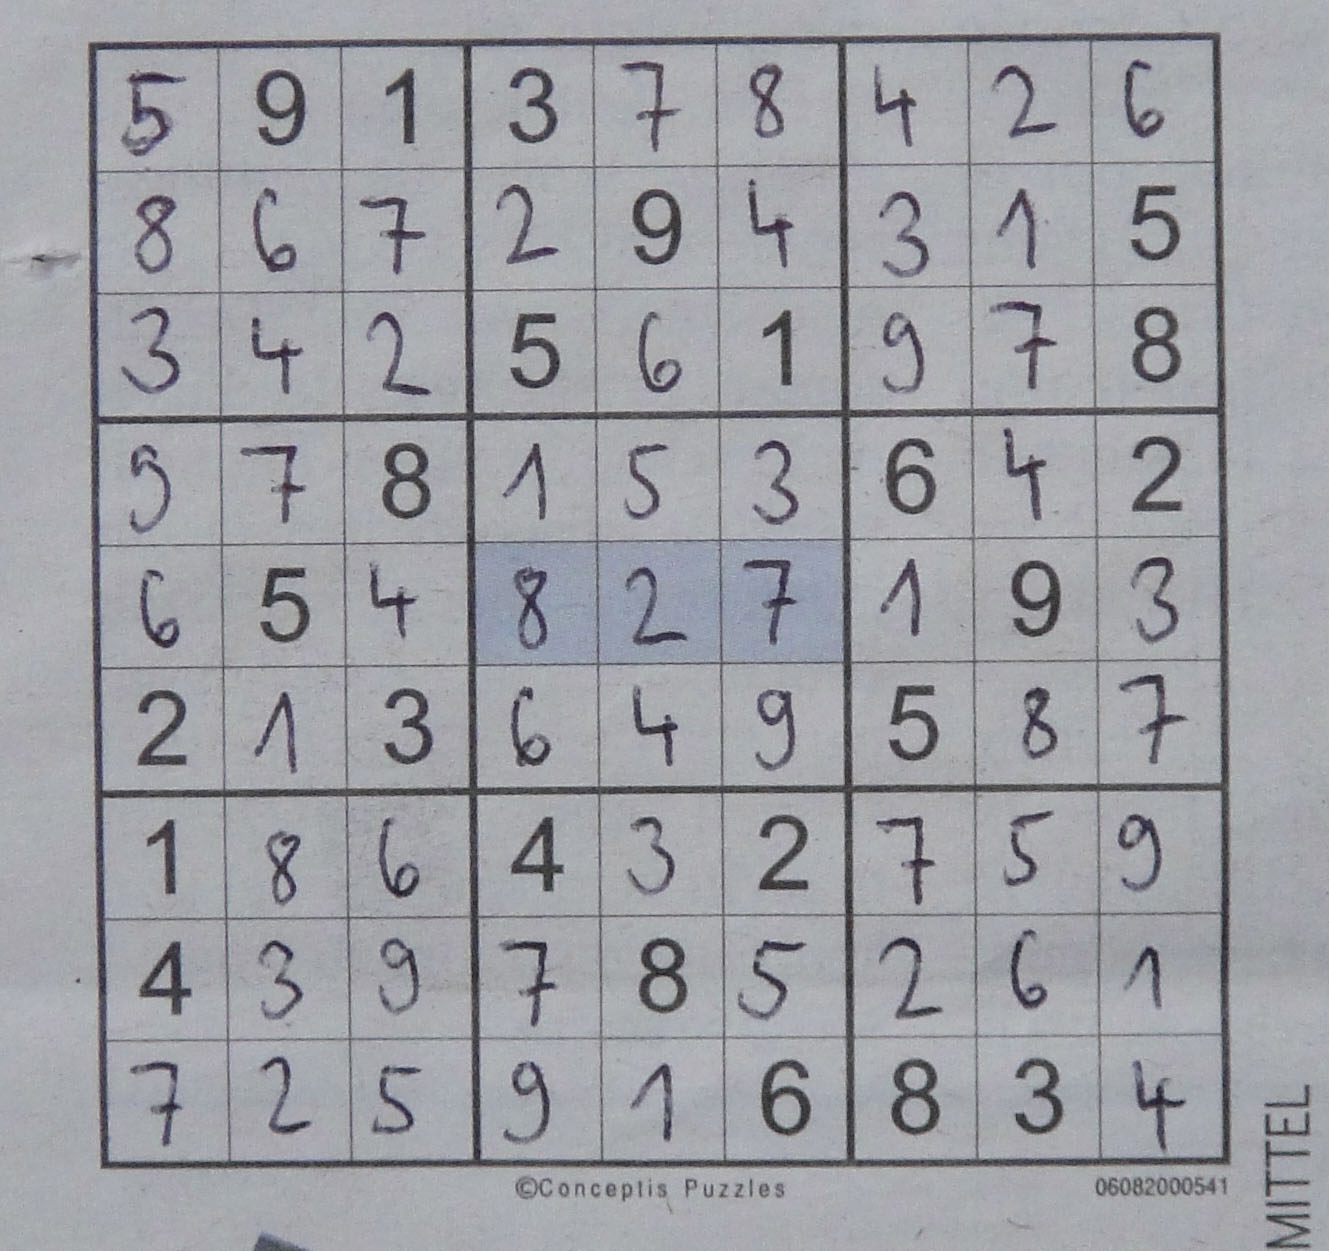
\includegraphics[width=0.5\textwidth]{sudoku_ausgefuellt.jpg}

\vfill

\hfill \scriptsize{source: 20 Minuten, 30.3.2010.}

\end{frame}


\section{Conclusion}

\begin{frame}
\frametitle{Conclusion}

\begin{itemize}[<+->]
    \item R is a high level statistical package
    \item R is versatile and can be adjusted for different needs
    \item \structure<3->{You should use R for your statistical analysis}
\end{itemize}

\end{frame}


\begin{frame}
\frametitle{Bibliography}

\scriptsize

\begin{thebibliography}{3}
\bibitem{Perez2008}
Meir Perez and Tshilidzi Marwala (2008)
\newblock Stochastic optimization approaches for solving sudoku
\newblock Int. Workshop on Stochastic and Applied Global Optimization: Skukuza, South Africa

\bibitem{R2009}
R Core Developer Team (2009)
\newblock The R project for statistical computing
\newblock \texttt{www.r-project.org}

\bibitem{Yang2010}
Ziheng Yang (2010)
\newblock Sudoku via simulated annealing
\newblock http://xianblog.wordpress.com/2010/02/23/sudoku-via-simulated-annealing/
\end{thebibliography}

\end{frame}


\begin{frame}

\centering
\huge
Questions ?!

\end{frame}


\end{document}
